\documentclass[a4paper,12pt]{extarticle}
\usepackage{geometry}
\usepackage[T1]{fontenc}
\usepackage[utf8]{inputenc}
\usepackage[main=english,russian]{babel}
\usepackage{amsmath}
\usepackage{amsthm}
\usepackage{amssymb}
\usepackage{fancyhdr}
\usepackage{setspace}
\usepackage{graphicx}
\usepackage{colortbl}
\usepackage{tikz}
\usepackage{pgf}
\usepackage{subcaption}
\usepackage{listings}
\usepackage{indentfirst}
\usepackage[
backend=biber,
style=numeric,
urldate=long,
maxbibnames=99
]{biblatex}
\addbibresource{refs.bib}
\usepackage[colorlinks,citecolor=blue,linkcolor=blue,bookmarks=false,hypertexnames=true, urlcolor=blue]{hyperref} 
\usepackage{indentfirst}
\usepackage{mathtools}
\usepackage{booktabs}
\usepackage[flushleft]{threeparttable}
\usepackage{tablefootnote}

\usepackage{chngcntr} % нумерация графиков и таблиц по секциям
\counterwithin{table}{section}
\counterwithin{figure}{section}

\graphicspath{{graphics/}}%путь к рисункам

\makeatletter
% \renewcommand{\@biblabel}[1]{#1.} % Заменяем библиографию с квадратных скобок на точку:
\makeatother

\geometry{left=2.5cm}% левое поле
\geometry{right=1.0cm}% правое поле
\geometry{top=2.0cm}% верхнее поле
\geometry{bottom=2.0cm}% нижнее поле
\setlength{\parindent}{1.25cm}
\renewcommand{\baselinestretch}{1.5} % междустрочный интервал


\newcommand{\bibref}[3]{\hyperlink{#1}{#2 (#3)}} % biblabel, authors, year
\addto\captionsrussian{\def\refname{Список литературы (или источников)}} 

\renewcommand{\theenumi}{\arabic{enumi}}% Меняем везде перечисления на цифра.цифра
\renewcommand{\labelenumi}{\arabic{enumi}}% Меняем везде перечисления на цифра.цифра
\renewcommand{\theenumii}{.\arabic{enumii}}% Меняем везде перечисления на цифра.цифра
\renewcommand{\labelenumii}{\arabic{enumi}.\arabic{enumii}.}% Меняем везде перечисления на цифра.цифра
\renewcommand{\theenumiii}{.\arabic{enumiii}}% Меняем везде перечисления на цифра.цифра
\renewcommand{\labelenumiii}{\arabic{enumi}.\arabic{enumii}.\arabic{enumiii}.}% Меняем везде перечисления на цифра.цифра

\begin{document}
\input{title_kr}% это титульный лист - выберите подходящий вам из имеющихся в проекте вариантов (kr - курсовая работа у 3 курса, vkr - выпускная квалификационная работа у 4 курса)
\newpage
\setcounter{page}{2}

{
	\hypersetup{linkcolor=black}
	\tableofcontents
}

\newpage

\newpage
\section*{Annotation} 
\addcontentsline{toc}{section}{Annotation}  % add Annotation to Table of Contents

Deep neural network--based solutions have been widely adopted in various audio processing applications. 
In particular, they are used in speech enhancement, where the goal is to remove background noise and enhance
the target speech signal. A key practical challenge of neural approaches is their high computational and 
memory cost, which becomes especially important under real-time constraints. 

In this work, we explore the use of FastGRNN blocks, which allow us to reduce the number of parameters by 40\%
while maintaining similar performance. We also experiment with redistributing parameters and test 
different convolutional blocks, including variants with the Affine PReLU activation.

\section*{\foreignlanguage{russian}{Аннотация}}   % this is how to use russian
\foreignlanguage{russian}{
Решения на основе глубоких нейронных сетей уже достаточно давно используются в различных приложениях,
связанных с обработкой звука. В частности, они применяются в задаче усиления речи (Speech Enhancement),
где требуется убрать шум из аудио и усилить основной речевой сигнал. Актуальной проблемой при использовании
нейросетевых решений на практике являются большие требования к вычислительным ресурсам и памяти, что вместе
с необходимостью работы в реальном времени становится серьёзным ограничением.

В данной работе мы рассматриваем использование FastGRNN блоков, что позволяет уменьшить число параметров примерно
на 40\% при сохранении близкого качества. Также мы исследуем перераспределение параметров между частями модели
и тестируем различные сверточные блоки, включая варианты с функцией активации Affine PReLU.
}

\section*{Keywords}
DL, Speech Enhancement, Noise Reduction, Deep Filtering
\pagebreak

\section{Introduction}

Speech enhancement is a well-known problem in audio signal processing. Its goal is to improve the quality and
intelligibility of speech signals degraded by noise, reverberation, or other distortions. In practice, speech enhancement methods should operate in real time with low latency on CPUs or low-power
devices, such as hearing aids and mobile phones. This requirement favors algorithms with a small memory
footprint, which is why many works focus on reducing the parameter count. Latency is another crucial factor,
especially in interactive scenarios, because large delays are noticeable and degrade user experience;
therefore, it also constrains architectural choices. Computational cost is also important, since the
method must run on limited hardware

Common approaches include traditional signal processing methods and, more recently, deep learning-based
techniques. Traditional methods such as spectral subtraction, Wiener filtering, and statistical model-based
approaches have been widely used for speech enhancement~\cite{bookse}. Today, these techniques are often used as components
of more complex systems, which we discuss later.

Deep learning approaches have significantly improved the quality of speech enhancement. However, many of them rely on 
large models that are difficult to deploy on resource-constrained devices. This makes the problem of building efficient 
models especially important.

One of the successful approaches in this direction is DeepFilterNet~\cite{dfn}, which combines a compact neural network with a
lightweight filtering stage. It provides a good balance between quality and efficiency and serves as a strong baseline
for real-time speech enhancement.

At the same time, further reduction of model complexity remains an open problem. Most existing works focus on modifying
the overall architecture or improving the training procedure. In contrast, the efficiency of recurrent blocks inside
such models and the distribution of parameters between different components are less explored.

In this work, we study how to reduce the complexity of DeepFilterNet while keeping the performance at a similar level.
We consider two directions: replacing GRU blocks with more parameter-efficient alternatives and rebalancing parameters
between the encoder--decoder and the deep filtering components.

The main contributions of this work are as follows:
\begin{itemize}
    \item We implement the DeepFilterNet model in PyTorch and reproduce its training pipeline on the VCTK+DEMAND dataset~\cite{vctk}.
    \item We evaluate the use of ComFi-FastGRNN~\cite{fastulcnet} (later we name it FastGRNN for simplicity) as a replacement for GRU blocks and show that it significantly reduces
	the number of parameters with only a small drop in performance.
    \item We study the effect of parameter rebalancing and show that the original configuration of DeepFilterNet is
	close to optimal in terms of quality.
    \item We analyze the trade-off between model quality and computational efficiency across different architectural
	modifications.
\end{itemize}

Our implementation is available at \url{https://github.com/runtime57/speech_enhancement}. This research was supported in
part through computational resources of HPC facilities at HSE University


\section{Related Work}

\subsection{Lightweight Speech Enhancement}

A widely used lightweight baseline in speech enhancement is RNNoise~\cite{rnnoise}, proposed by Valin. It partitions the
spectrum into Bark-scale bands and uses a small recurrent network to estimate an ideal ratio mask (IRM) for each band.
In addition, it applies a pitch-filtering module to suppress noise between harmonics. 

The method is highly efficient in terms of computational cost and memory footprint, but it is typically outperformed
by modern approaches on quality metrics. Nevertheless, recurrent architectures remain widely used in speech enhancement,
as they are well suited for modeling sequential signals such as audio.

A summary of the discussed models and their main characteristics is shown in Table~\ref{table:models}.

\subsection{DeepFilterNet}

Lightweight hierarchical RNNs are a main focus of Schr\"oter et al.~\cite{dfn}. The authors introduce DeepFilterNet,
an efficient real-time speech enhancement framework.

DeepFilterNet operates in the STFT (time--frequency) domain and uses a compact neural backbone to extract spectral
features and predict a suppression mask that attenuates noise across time and frequency. To improve quality without
a large increase in computation, the model also predicts coefficients for a lightweight learnable complex filtering
step (``deep filtering''), which refines the enhanced spectrum and reduces residual artifacts. The enhanced waveform
is reconstructed via the inverse STFT.

DeepFilterNet has become an influential solution and inspired several follow-up works. For example, DeepFilterNet2
~\cite{dfn2} improves the original model mainly through better training procedures and data augmentation. Another
extension targets hearing aid applications and studies the integration of classical filters such as Wiener and MVDR
into the framework.

\subsection{Architectural Extensions}

Several works explore modifications of the DeepFilterNet architecture. One example is DPDFNet~\cite{dpdfnet}, where
the authors replace standard RNN blocks with Dual-Path RNN (DPRNN) blocks. The overall design remains similar to
DeepFilterNet, but the dual-path structure allows separate modeling of temporal and frequency dependencies.

A similar idea is used in Hierarchical DFNet~\cite{hdfnet}, where the model is split into two components: a coarse
spectral enhancement network and a temporal enhancement network. The authors achieve a very low parameter count while
maintaining competitive performance. This reflects a broader trend of replacing or restructuring recurrent components
to improve efficiency.

\subsection{Research Gap}

Most existing works focus on modifying the overall architecture or improving the training procedure. However, relatively
little attention is given to improving the efficiency of recurrent blocks inside such models.

Some recent works, such as Fast ULCNet~\cite{fastulcnet}, explore the use of more efficient recurrent architectures for
speech enhancement and show that significant parameter reduction is possible. However, such approaches are not studied
in the context of DeepFilterNet and similar hybrid architectures.

In particular, the effect of replacing standard GRU units with more parameter-efficient alternatives in DeepFilterNet
remains underexplored. Additionally, there is limited analysis of how parameter allocation between different parts of
the model affects performance.

In this work, we address these questions by studying the use of FastGRNN-based units in DeepFilterNet and by analyzing
the effect of rebalancing parameters between the encoder--decoder and the deep filtering components.

\begin{table}[h]
	\caption{Comparison of named models. Dataset: VCTK+DEMAND. Metrics were adopted from~\cite{hdfnet},~\cite{dpdfnet}.}
	\label{table:models}
	\footnotesize
	\centering
	\begin{tabular}{lccccccc}		
	\toprule
	 & $\mathsf{Para.(M)}$ & $\mathsf{MACs(G/s)}$ & $\mathsf{PESQ}$ & $\mathsf{STOI}$ & $\mathsf{CSIG}$ & $\mathsf{CBAK}$ & $\mathsf{COVL}$ \\
	\midrule
	RNNoise & 0.06 & 0.04 & 2.34 & 88.5 & 3.40 & 2.51 & 2.84 \\
	DeepFilterNet & 1.78 & 0.35 & 2.81 & - & 4.14 & 3.31 & 3.46 \\
	HDF-Net & 0.20 & 0.43 & 3.01 & - & 4.24 & 3.52 & 3.64 \\
	DPDFNet & 3.54 & 4.37 & 2.90 & 93.4 & - & - & - \\
	\bottomrule
	\end{tabular}
\end{table}


\section{Methodology}

\subsection{Signal model}

Let $s(t) \in \mathbb{R}^{N \times T}$ be the clean speech signal, where $N$ is the number of channels
and $T$ is the number of time stamps. The noisy observation $x(t)$ can be represented as

\[
x = s * h + \epsilon,
\]

where $h$ is the room impulse response from the speaker to the microphone and $\epsilon$ is additive noise.

We operate in the short-time Fourier transform (STFT) domain since spectral transforms are
an expressive feature transform allowing for smaller parameter counts.
Under a standard narrowband approximation, the model can be written as

\[
X(k, f) = S(k, f)H(k, f) + N(k, f),
\]

where $S(k, f)$ is the STFT of the clean speech, $N(k, f)$ is the STFT representation of the additive 
noise, $k$ is the time-frame index, and $f$ is the
frequency-bin index. The same notation applies to $X(k, f)$, $H(k, f)$, and $N(k, f)$.

\subsection{Original DeepFilterNet architecture}

Full framework of DeepFilterNet is illustrated in Fig.~\ref{fig:dfnet}. We apply STFT to the noisy 
audio signal $x(n)$ and then observe two types of features.
$X_{\mathsf{ERB}} (k, b)$, where $b \in [0, \mathsf{N_{ERB}}]$  and $\mathsf{N_{ERB}}$ is a number of bands. 
To extract ERB features, we first compute the STFT magnitude and convert it to log-power representation. 
Then, frequency bins are grouped into perceptual bands using an ERB filter bank.

The resulting features are normalized using an exponential moving average over time. This provides a 
compressed and stable representation of the spectrum, reducing dimensionality while preserving important
speech information, which helps the model focus on relative spectral changes rather than absolute signal level.

The second type of features DeepFilterNet uses is standard complex spectrogram $X_{\mathsf{DF}}$. An exponential unit 
normalization is applied. Complex features are passed to the deep filter network.

DeepFilterNet follows an encoder-decoder architecture to predict ERB-domain gains. These gains are then
mapped back to the frequency domain using an inverse ERB filter bank and applied to the noisy spectrogram
by pointwise multiplication.

To further refine the result, the model predicts complex-valued deep filtering coefficients of order $N$.
These coefficients are applied in the STFT domain and help improve periodic components of speech. In
practice, deep filtering is only used up to a cutoff frequency $f_{\mathrm{DF}}$, since most periodic
speech energy is concentrated in lower frequencies.

The neural network itself is designed to be efficient and uses only standard building blocks such as
convolutions, batch normalization, and ReLU activations. The authors suggest adopting a U-Net-like architecture with encoder
and decoder pathways connected by skip connections, which helps preserve frequency resolution.

The convolutional blocks are based on separable convolutions (depthwise followed by $1 \times 1$ convolution).
The layers are arranged in time such that only the first layers introduce a small look-ahead
$l_{\mathrm{DNN}}$, while the remaining layers are causal and do not increase latency.

For the recurrent and linear layers, grouped computation is used to reduce complexity. The input is split into
$P$ groups, processed independently, and then combined back. This allows the model to maintain a relatively
large hidden size while keeping the computational cost low.

Finally, additional skip connections are used to preserve information about the original noisy phase, which
improves the quality of the reconstructed signal.

\begin{figure}[ht]
	\centering
	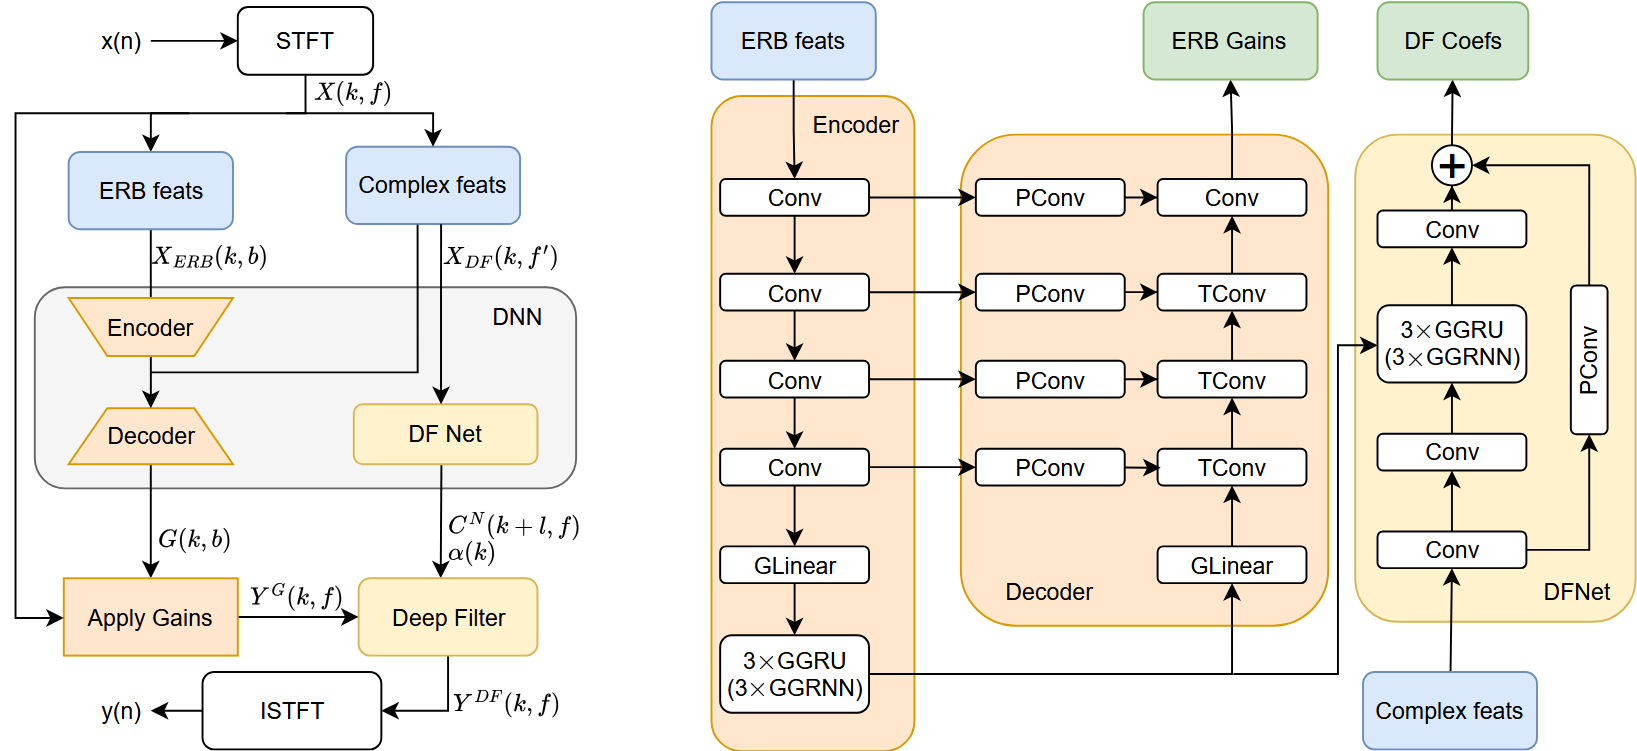
\includegraphics[width=1\textwidth]{full_colored.png}
	\caption{This illustration shows full DeepFilterNet framework. GLinear and GGRU (GGRNN) refer to the grouped blocks 
	of Linear, GRU (FastGRNN) layers. Inspired by~\cite{dfn}.}
	\label{fig:dfnet}
\end{figure}

\subsection{FastGRNN block}

Our main approach is to replace GRU blocks with Comfi-FastGRNN blocks that were proposed in~\cite{fastulcnet}. This
allows us to lower the number of parameters without a significant drop in performance. The architecture of
the block is shown in Fig.~\ref{fig:fastgrnn}.

\begin{figure}[ht]
	\centering
	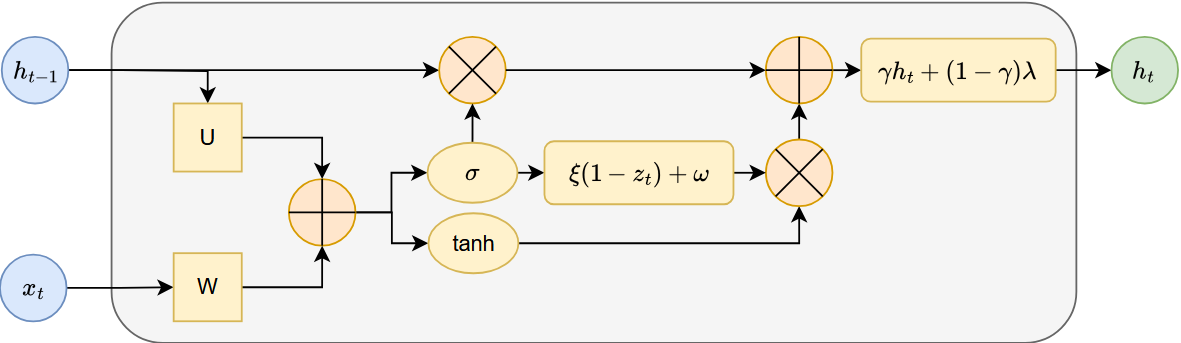
\includegraphics[width=1\textwidth]{fastgrnn.png}
	\caption{This illustration shows full Comfi-FastGRNN block. Inspired by~\cite{fastulcnet}.}
	\label{fig:fastgrnn}
\end{figure}

FastGRNN uses a gated update with a residual connection. The hidden state is updated as
\begin{align}
z_t &= \sigma(Wx_t + Uh_{t-1} + b_z), \\
\tilde{h}_t &= \tanh(Wx_t + Uh_{t-1} + b_h), \\
h_t &= (\xi(1 - z_t) + \omega)\odot \tilde{h}_t + z_t \odot h_{t-1},
\end{align}
where $\xi, \omega \in [0, 1]$ are learnable scalar parameters. This design reduces the number of parameters
and stabilizes training.

However, when applied to long sequences, FastGRNN may suffer from drift in the hidden state during inference.
To address this, ComFi-FastGRNN introduces a correction term and modifies the update as
\begin{equation}
h_t^{\text{comfi}} = \gamma h_t + (1 - \gamma)\lambda,
\end{equation}
where $\gamma$ controls the contribution of the original hidden state and $\lambda$ is a learnable vector.

This modification helps to prevent accumulation of errors over time and results in more stable behavior,
while keeping the model lightweight.

\subsection{Convolutional blocks}

Inspired by a recent paper, we also experiment with several types of convolutional blocks that have shown the best results in~\cite{ulunas}.
Still, we have to make some changes to adapt the blocks to DeepFilterNet framework.

First, we adapt all convolutional layers to match the original DeepFilterNet geometry. In particular, we use asymmetric kernels of the form 
$(k_t,k_f)$, where the frequency dimension is fixed to $3$ when an integer kernel size is provided. This follows the convention used 
in DeepFilterNet and ensures compatibility with ERB features.

In addition, we control causality in convolutional layers using manual temporal padding. A look-ahead parameter defines the amount
of future context and therefore the latency.

We use three types of blocks:
\begin{itemize}
    \item \textbf{Conv:} standard convolution $\to$ BN $\to$ activation, used as a baseline block in~\cite{ulunas}.
    \item \textbf{DWS:} pointwise convolution followed by depthwise convolution for efficient channel and spatial processing~\cite{mobilenets}.
    \item \textbf{MB:} inverted residual design introduced in MobileNetV2~\cite{mobilenetv2}.
\end{itemize}

All the architectures are illustrated in Fig.~\ref{fig:blocks}.

\begin{figure}[ht]
	\centering
	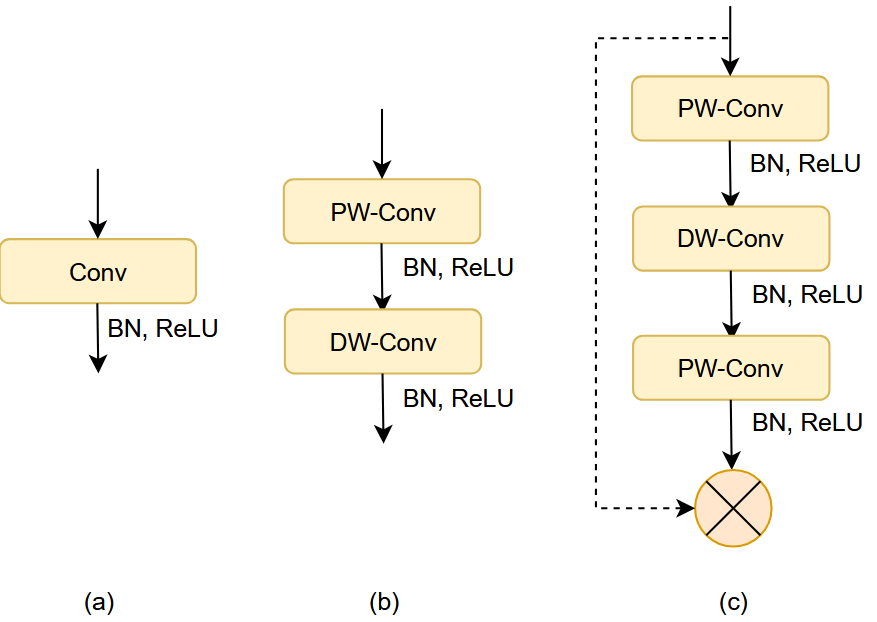
\includegraphics[width=0.75\textwidth]{blocks.png}
	\caption{This illustration shows the architecture of the used blocks: (a) Conv (b) DWS (c) MB. Inspired by~\cite{ulunas}.}
	\label{fig:blocks}
\end{figure}

\subsection{Affine PReLU}

\paragraph{Affine PReLU}
We use Affine PReLU (APReLU) proposed in~\cite{ulunas}, which extends standard PReLU by adding a learnable affine
transformation. The activation is defined as
\[
h(x) = \gamma x + \beta + \text{PReLU}(x),
\]
where $\gamma$ and $\beta$ are learnable parameters that depend on channel and frequency. This allows the model to
adapt feature scaling across frequency bands, which is important for speech signals.



\subsection{Loss}

The total loss is defined as a combination of two terms:
\begin{equation}
\mathcal{L} = \lambda_{\text{spec}} \cdot \mathcal{L}_{\text{spec}}(Y, S) + \lambda_{\alpha} \cdot \mathcal{L}_{\alpha},
\end{equation}
where $\mathcal{L}_{\text{spec}}$ is a spectral reconstruction loss and $\mathcal{L}_{\alpha}$ is an additional term controlling the contribution of the deep filtering component.

\paragraph{Spectral loss}

The spectral loss is computed in the STFT domain and compares the enhanced signal $Y$ with the clean signal $S$. It consists of two parts: a magnitude term and a phase-aware term:
\begin{equation}
\mathcal{L}_{\text{spec}} =
\sum_{k,f} || |Y(k,f)|^c - |S(k,f)|^c ||^2
+
\sum_{k,f} || |Y(k,f)|^c e^{j\varphi_Y(k,f)} - |S(k,f)|^c e^{j\varphi_S(k,f)} ||^2,
\end{equation}
where $c$ is a compression factor.

The first term compares magnitudes and encourages correct spectral envelope reconstruction. The second term additionally takes phase into account by comparing complex-valued spectra.

\paragraph{Angle-aware stabilization}

To improve stability for time--frequency bins with small magnitude, the phase term is computed using a normalized representation:
\begin{equation}
\frac{\partial \varphi}{\partial X} = \delta X \cdot ( -\frac{\Im\{X\}}{|X_h|^2}, \frac{\Re\{X\}}{|X_h|^2} ),
\end{equation}
where $|X_h|^2 = \max(|X|^2, \varepsilon)$ is a stabilized magnitude.

\paragraph{Deep filtering control term}

The second part of the loss controls where deep filtering should be applied. It is defined as
\begin{equation}
\mathcal{L}_{\alpha} =
\sum_k || \alpha \cdot \mathbf{1}_{\text{LSNR} < -10\text{ dB}} ||^2
+
\sum_k || (1 - \alpha) \cdot \mathbf{1}_{\text{LSNR} > -5\text{ dB}} ||^2,
\end{equation}
where LSNR is the local signal-to-noise ratio.

This term encourages the model to apply deep filtering mainly in regions where speech is present and avoids using it in noise-only segments.

\subsection{Evaluation metrics}

In addition to computational efficiency metrics such as parameter count and MACs (Multiply–Accumulate Operations), we use several quality
metrics to evaluate our model. For 16 kHz speech enhancement, widely used objective metrics include PESQ
(Perceptual Evaluation of Speech Quality)~\cite{pesq} and STOI (Short-Time Objective Intelligibility)~\cite{stoi}.

PESQ measures perceived speech quality by comparing the enhanced signal with a clean reference. STOI
focuses on intelligibility and shows how good speech content is after enhancement.

We also report SI-SDR (scale-invariant signal-to-distortion ratio). This metric measures similarity between enhanced and clean signals
and is invariant to scaling, which makes it suitable for model comparison.

Using several metrics helps evaluate different aspects of performance, since improvements in one metric do
not always lead to improvements in others.

We measure MACs using thop Python library.


\section{Experimental setup}

\subsection{Datasets}

Unlike the DeepFilterNet authors, we use the VCTK dataset~\cite{vctk} instead of the original DNS Challenge
dataset~\cite{dns}. In particular, we use a noisy speech database designed for training speech enhancement algorithms and
TTS systems. The dataset is constructed using noise samples from the DEMAND dataset~\cite{demand}, therefore in most
papers it is referred to as VCTK+DEMAND. It is widely used in speech enhancement research as a standard
benchmark, which allows for direct comparison between different methods. For example, it is commonly used
in works evaluating lightweight and real-time speech enhancement models.

The dataset consists of clean speech recordings from the VCTK corpus~\cite{vctkcorpus}, which contains speech from multiple
speakers with diverse accents, and corresponding noisy versions obtained by mixing with environmental noise.
The noise signals are taken from the DEMAND dataset and include a variety of real-world acoustic conditions,
such as domestic, office, and outdoor environments.

The major difference from the DNS dataset is that by choosing VCTK, we do not generate noisy recordings on-the-fly
during training, but instead use pre-generated pairs of clean and noisy signals. This simplifies the training
pipeline and ensures reproducibility of experiments, but at the same time reduces flexibility in terms of
noise sampling and mixing strategies compared to DNS-based approaches.

The data is available in several sampling rates: 28 kHz, 48 kHz, and 56 kHz. However, we use the 48 kHz
version and resample it to 16 kHz, since many evaluation metrics are defined for this sampling rate. In
addition, working at 16 kHz reduces computational cost and is consistent with typical real-time deployment
scenarios on resource-constrained devices.

We use the official train/test split. The training set consists of 11572 samples and the
evaluation set consists of 824 samples.

\subsection{Baselines}

\textbf{Original DeepFilterNet.} We ran the original DeepFilterNet pipeline 
on our evaluation set.

However, we cannot directly compare our results with the original paper, since the training data 
differs significantly and the training setup is not the same in terms of both data generation and 
computational budget.


Therefore, this experiment serves as a reference point rather than a strict baseline. The main 
comparisons in this work are performed with our own implementation of the model. Still, it is useful
to see how the training setup affects the metrics

\textbf{Our implementation of DeepFilterNet.} Since the authors of the original paper later focused on 
frameworks for hearing aid devices, their public implementation includes several optimizations, such as a 
custom Rust-based framework for the training process (dataloader, datasets, etc.).

Our implementation is done in PyTorch and is fully written in Python. All further baselines are also 
implemented within our template, so the main comparison is performed with this model.

This version is trained from scratch on the VCTK+DEMAND dataset and evaluated on the official 
evaluation set. All hyperparameters are kept the same as in the original DeepFilterNet. This ensures that 
differences in performance are mainly due to the implementation and training setup rather than hyperparameter
changes.

\textbf{FastDeepFilterNet.} For this baseline, we replace GRU blocks with Comfi-FastGRNN units. To the best of
our knowledge, this is one of the first works in speech enhancement that explores the use of FastGRNN in this
setting, which makes this experiment relevant.

We keep the original dimensions of DeepFilterNet and expect to reduce the number of parameters due to the
more efficient structure of Comfi-FastGRNN, while keeping the metrics at approximately the same level.

We evaluate whether replacing standard recurrent units with more
parameter-efficient ones can improve the overall trade-off between model size and performance.

At the same time, this modification may affect temporal modeling, which we evaluate in the
experiments.

\textbf{Rebalanced DeepFilterNet.} We train three different versions of a rebalanced model. The key idea here is to
concentrate more parameters in the deep filtering part rather than in the encoder--decoder. By this shift of focus,
we aim to achieve higher metrics with approximately the same number of parameters. 

The intuition behind these experiments is that the deep filtering stage is responsible for denoising and 
reconstruction of harmonic structure. Therefore, increasing its capacity may lead to better performance, 
especially in STOI and PESQ metrics, which reflect perceived speech quality and intelligibility.

At the same time, reducing the capacity of the encoder--decoder may negatively affect feature extraction
quality, which can limit the overall performance of the model.

Table~\ref{table:rebalanced} shows the configurations of our experiments. The models are numbered from 1 
to 3 based on how aggressive the rebalancing is (higher numbers correspond to a stronger shift of 
parameters towards the deep filtering part).

\begin{table}[h]
	\caption{Concrete hyperparameters for rebalanced models.}
	\label{table:rebalanced}
	\footnotesize
	\centering
	\begin{tabular}{lcccccc}		
	\toprule
	 & $\mathsf{ch_{conv}}$ & $\mathsf{H_{emb}}$ & $\mathsf{N_{emb}}$ & $\mathsf{H_{df}}$ 
	 & $\mathsf{N_{df}}$ & $\mathsf{Params (M)}$ \\
	\midrule
	Original & 64 & 512 & 3 & 512 & 2 & 1.69 \\
	Rebalanced-1 & 48 & 512 & 3 & 576 & 2 & 1.03 \\
	Rebalanced-2 & 40 & 512 & 3 & 640 & 2 & 1.09 \\
	Rebalanced-3 & 32 & 512 & 3 & 704 & 2 & 1.15 \\
	\bottomrule
	\end{tabular}
\end{table}

\textbf{Convolutional blocks experiments.} We also compare different convolutional blocks. The baselines are named
DWS, MB and Conv for basic versions, and XDWS, XMB, XConv for versions with APReLU. We integrate all these blocks into
the FastDeepFilterNet model that uses FastGRNN modules.

The goal is to evaluate the trade-off between computational efficiency and model performance. In particular, we study
whether these blocks can improve quality at low additional cost.


\subsection{Training}


The training setup is the same for all baselines. We use the AdamW optimizer with a learning rate of $1\mathrm{e}{-3}$.
A StepLR scheduler is applied with $\gamma = 0.9$. One epoch corresponds to a full pass over the training set with a
batch size of 32. Zero-padding is applied using the input padding mode.

The model operates in the STFT domain. We use a sampling rate of 16 kHz with an FFT size of 320 and a hop length of
160, corresponding to a 50\% overlap. For ERB features, we use 24 bands, while the deep filtering stage operates on
96 frequency bins.

Feature normalization is performed using an exponential moving average with time constant $\tau = 1$. The local SDR
is clipped to the range $[-15, 35]$ dB to stabilize training. The deep filtering module uses a filter order of 5
with a look-ahead of 1 frame.


You can find all the configurations in our official repository.



\subsection{Results}


\subsubsection{Our models}

\begin{table}[h]
	\caption{Results of evaluating the models on the VCTK+DEMAND dataset. Best results are shown in bold, second-best are underlined.}
	\label{table:results}
	\footnotesize
	\centering
	\begin{tabular}{lccccc}
	\toprule
	& $\mathsf{Params\ (M)\ \downarrow}$ 
	& $\mathsf{MACs\ (G)\ \downarrow}$ 
	& $\mathsf{PESQ\ \uparrow}$ 
	& $\mathsf{STOI\ \uparrow}$ 
	& $\mathsf{SI\text{-}SDR\ \uparrow}$\\
	\midrule
	Original DFNet & 1.78      & 0.35      & \bf{2.81} & \bf{0.94} & 16.63     \\
	\midrule
	Our DFNet      & 1.69      & 0.51      & \underline{2.31} & \underline{0.93} & \bf{17.04} \\
	FastDFNet      & \underline{1.04} & 0.34      & 2.26      & \underline{0.93} & \underline{17.00}      \\
	Rebalanced-1   & \bf{1.03} & 0.25      & 2.21      & 0.92 & 16.53      \\
	Rebalanced-2   & 1.09      & \underline{0.21} & 2.24      & 0.92 & 16.83      \\
	Rebalanced-3   & 1.15      & \bf{0.19} & 2.16      & 0.92 & 16.49      \\
	\midrule
	DWS       & \underline{1.04} & \underline{0.32} & 2.25      & \underline{0.93} & 16.86      \\
	MB        & 1.08      & 0.52      & 2.24      & \underline{0.93} & 16.96      \\
	Conv      & 1.11      & 0.68      & 2.25      & \underline{0.93} & 16.97      \\
	\midrule
	XDWS      & 1.11      & \underline{0.32} & 2.24      & 0.92 & 16.71      \\
	XMB       & 1.17      & 0.50      & 2.25      & \underline{0.93} & 16.79      \\
	XConv     & 1.12      & 0.68      & 2.26      & \underline{0.93} & 16.77      \\
	\bottomrule
	\end{tabular}
\end{table}

Our implementation of DeepFilterNet serves as the main internal baseline for all further experiments. This confirms that our
implementation is valid and suitable as a baseline. Direct comparison with the official implementation is
limited, as discussed above.
The difference in MACs is likely due to differences in measurement methodology and implementation details.

The results are shown in Table~\ref{table:results}. Replacing GRU blocks with Comfi-FastGRNN leads to a significant reduction in the number of parameters (from 1.69M to 1.04M),
while the drop in metrics is relatively small. In particular, STOI remains unchanged, and the decrease in PESQ and SI-SDR 
is limited. We can conclude that FastGRNN is an effective lightweight alternative to GRU, although it slightly reduces the
model's ability to capture temporal dependencies.

The rebalanced models do not show improvement in metrics despite reallocating parameters towards the deep filtering stage.
As the rebalancing becomes more aggressive, performance gradually decreases, which indicates that increasing the capacity of
the deep filtering component alone is not sufficient to improve overall quality.

The reason may be that the encoder--decoder part of the model plays an important role in extracting meaningful
spectral features. Reducing its capacity leads to weaker representations, which cannot be compensated for by a more powerful
deep filtering stage.

At the same time, we observe a consistent reduction in computational cost for the rebalanced models. MACs
decrease as more parameters are shifted towards the deep filtering part. Although the rebalancing
does not improve quality metrics, it provides a more efficient model in terms of computation.

Both experiments confirm that changing the architecture without carefully preserving the balance between representation
learning and signal reconstruction may lead to performance degradation.

Finally, we analyze the effect of convolutional blocks. DWS provides the best efficiency with lower MACs, while MB and
Conv offer slightly better quality at higher cost. This indicates that convolutional design plays a secondary role
compared to recurrent modeling in DeepFilterNet.

The use of Affine PReLU (X-blocks) does not lead to consistent improvements. It shows that activation modification alone is not sufficient in this setup.

Overall, the best trade-off between quality and efficiency is achieved by FastDFNet and DWS-based variants. This
confirms that lightweight architectural changes are more effective than increasing model complexity for this task.

\subsubsection{Comparison with other models}

\begin{table}[h]
	\caption{Performance comparison on the VCTK+DEMAND dataset. Best results are shown in bold, second-best are underlined. SI-SDR is used as an approximation of SI-SNR for comparison. The metrics were adopted from~\cite{ulunas}.}
	\label{table:other}
	\footnotesize
	\centering
	\begin{tabular}{lccccc}
	\toprule
	& $\mathsf{Params\ (M)\ \downarrow}$ 
	& $\mathsf{MACs\ (G)\ \downarrow}$ 
	& $\mathsf{PESQ\ \uparrow}$ 
	& $\mathsf{STOI\ \uparrow}$ 
	& $\mathsf{SI\text{-}SDR\ \uparrow}$\\
	\midrule
	Noisy           & -      & -      & 1.97      & 0.921 & 8.45 \\
	RNNoise         & \underline{0.06}   & \underline{0.04}   & 2.29      & -     & - \\
	PercepNet       & 8.00   & 0.80   & 2.73      & -     & - \\
	FullSubNet      & 5.64   & 30.87  & 2.89      & 0.940 & - \\
	DeepFilterNet   & 1.80   & 0.35   & 2.81      & \bf{0.942} & 16.63 \\
	GaGNet          & 5.95   & 1.65   & 2.94      & 0.940 & - \\
	FastFullSubNet  & 6.84   & 4.14   & 2.79      & 0.935 & - \\
	GTCRN           & \underline{0.05}   & \bf{0.03} & 2.87 & 0.940 & \bf{18.83} \\
	LiSenNet        & \bf{0.04} & 0.06 & 2.95 & 0.937 & - \\
	LiSenNet (+PESQ)& \bf{0.04} & 0.06 & \underline{3.07} & 0.939 & - \\
	UL-UNAS         & 0.17   & \bf{0.03} & 2.96 & \underline{0.941} & 18.25 \\
	UL-UNAS (+PESQ) & 0.17   & \bf{0.03} & \bf{3.09} & \underline{0.941} & \underline{18.48} \\
	\midrule
	Our DFNet       & 1.69   & 0.51   & 2.31      & 0.934  & 17.04 \\
	FastDFNet       & 1.04   & 0.34   & 2.26      & 0.924  & 17.00 \\
	Rebalanced-1    & 1.03   & 0.25   & 2.21      & 0.921  & 16.53 \\
	Rebalanced-3    & 1.15   & 0.19   & 2.16      & 0.922  & 16.49 \\
	DWS        & 1.04   & 0.32   & 2.25      & 0.928  & 16.86 \\
	\bottomrule
	\end{tabular}
\end{table}


We also provide a comparison with other models in Table~\ref{table:other}. The results show that modern lightweight 
architectures significantly outperform DeepFilterNet in terms of both efficiency and quality. In particular, 
UL-UNAS achieves the best PESQ (3.09) while maintaining very low computational cost (0.03 MACs), and GTCRN 
provides the best SI-SDR (18.83) with extremely small model size.

Although our models remain competitive within the DeepFilterNet family, there is still a noticeable gap between our
models and state-of-the-art methods. 

The results confirm that while DeepFilterNet can be made more efficient, but achieving state-of-the-art
performance requires more fundamental architectural changes.



\section{Plan of further work}

Our plans are to continue experimenting with different architectural choices.

First of all, we want to evaluate the use of GTCRN -- another RNN-based architecture that was introduced in~\cite{gtcrn} and is designed as a
part of an ultra-lightweight model for speech enhancement. The authors report high-quality results with only 27K
parameters. However, we need to reproduce the model and integrate it into our training pipeline before making a fair
comparison.

Secondly, there are a number of works that explore hierarchical versions of DeepFilterNet like ~\cite{hdfnet}. We plan to combine such
architectures with more efficient recurrent blocks, such as Comfi-FastGRNN or GTCRN, to further study the trade-off
between model capacity and performance.

Another direction of research is the use of the DNS 4 Challenge dataset, which is widely adopted in the speech
enhancement community. Evaluation on this dataset would allow for a more direct comparison with many recent models
that do not provide open-source implementations. However, at the current stage, such experiments are limited by
computational and storage constraints, as the dataset exceeds the available resources on the cHARISMA supercomputer. We
have already submitted a request to add the DNS dataset to list of available datasets.

Finally, we plan to explore the use of GAN-based modules to improve perceptual quality. In particular, adversarial
training may help the model better capture fine-grained structure of speech and reduce artifacts that are not well
addressed by standard spectral losses. This could lead to improvements in perceptual metrics such as PESQ, even if
signal-level metrics remain similar. At the same time, such approaches require careful balancing of the loss terms
and may increase training instability, which we plan to investigate.


\section{Conclusion}

In this work, we explored several lightweight modifications of DeepFilterNet. Replacing GRU with
FastGRNN significantly reduces the number of parameters while keeping similar quality. This makes it
a good option for resource-limited settings.

Rebalancing parameters towards the deep filtering part reduces computation but does not improve performance. This
suggests that the original balance between model components is already close to optimal.

Experiments with convolutional blocks show that changing local convolution structure has limited effect. The use
of APReLU also does not give consistent improvements.

Overall, DeepFilterNet can be made more efficient with simple changes. However, to reach state-of-the-art results,
more significant changes in the model design are needed.

\section*{Use of AI Tools}
AI tools (ChatGPT, GPT-5.3) were used to help with phrasing and as a better version of translator. At early stages,
they were also used to better understand the topic and related papers.

\newpage 
\printbibliography[heading=bibintoc]   % [] are for appearing in Table of Contents

\end{document}
